\documentclass[a4paper]{article}
\usepackage{media9}
\usepackage{graphicx}
\usepackage{animate}
\usepackage{wrapfig}
\usepackage{pgfplots}
\usepackage{float}
\usepackage{booktabs}

\author{Guillen, Youssef}
\title{Algoritmi di ordinamento e i loro casi di uso}
\begin{document}

\maketitle
\section*{Introduzione:}
In questo elaborato verrà illustrata la modalità d’uso dei vari algoritmi di ordinamento; con annessa misurazione del tempo che impiega un 
algoritmo ad ordinare \(N\) elementi.
\section{bubble sort:}
Il Bubble Sort è un algoritmo di ordinamento semplice e intuitivo che funziona confrontando coppie adiacenti di elementi in una lista e scambiandoli se sono 
\begin{wrapfigure}{r}{0.15\textwidth}
    \centering
    \animategraphics[loop,autoplay,scale=0.44]{10}{C:/Users/daniel/Desktop/algoritmi-ordinamento/relazione/media/Bubblesort/Bubblesort2-}{0}{207}
\end{wrapfigure}
nell'ordine sbagliato. Questo processo continua ripetutamente fino a quando l'intera lista è ordinata. L'algoritmo "fa salire" gli elementi 
più grandi (o più piccoli, a seconda dell'ordinamento desiderato) verso la fine della lista.
Il nome "Bubble" (bolla) deriva dal fatto che le coppie di elementi vengono inmagazzinati in delle bolle e poi scambiati se necessario.
Il funzionamento del Bubble Sort si articola in più passaggi. In ogni passaggio, l'algoritmo confronta coppie di elementi adiacenti e li scambia se il primo è 
maggiore (nel caso di ordinamento crescente) del secondo. Dopo ogni iterazione, l'elemento più grande è posizionato nella sua posizione corretta, quindi la parte 
della lista che deve essere ulteriormente esaminata diminuisce progressivamente. Il processo continua fino a quando non sono più necessari scambi, 
indicando che la lista è ordinata.
\subsection{Complessità:}
La complessità temporale del Bubble Sort è \(O(n^2)\) nel caso medio e nel caso peggiore. Questo perché, nel caso di una lista non ordinata, l'algoritmo 
effettua \(n-1\) confronti nel primo passaggio, \(n-2\) nel secondo, e così via. Di conseguenza, il numero totale di confronti è proporzionale a \(n^2\), il che 
rende l'algoritmo inefficiente per liste di grandi dimensioni. Tuttavia, nel caso migliore, quando la lista è già ordinata, l'algoritmo può essere ottimizzato
per terminare subito dopo una singola scansione, riducendo la complessità a \(O(n)\).
Il Bubble Sort viene spesso utilizzato in contesti educativi per insegnare i concetti di base degli algoritmi di ordinamento, grazie alla sua semplicità. Tuttavia, 
a causa della sua inefficienza, non è consigliato per l'ordinamento di grandi dataset.
\begin{figure}[h]
    \begin{tikzpicture}
        \begin{axis}[ 
            xlabel=$x$,
            ylabel=$y$,
            xmin=0,
            ymin=0,
            ] 
            \addplot {x^2}; 
        \end{axis}
    \end{tikzpicture}
    \caption{grafico dell'equazione della complessita del algoritmo bubble sort}
\end{figure}
\section{Selection Sort:}
\begin{wrapfigure}{r}{0.15\textwidth}
    \begin{center}
        \animategraphics[loop,autoplay,scale=0.44]{10}{C:/Users/daniel/Desktop/algoritmi-ordinamento/relazione/media/Selectionsort/Selectionsort2-}{0}{560}
    \end{center}
\end{wrapfigure}
Selection Sort è un algoritmo di ordinamento semplice che funziona selezionando ripetutamente l'elemento minimo (o massimo, a seconda del caso) dalla
 parte non ordinata della lista e spostandolo alla fine della parte ordinata. L'algoritmo suddivide la lista in due sezioni: una ordinata e una non ordinata. 
 Inizialmente, la parte ordinata è vuota, mentre la parte non ordinata contiene tutti gli elementi. Ogni iterazione dell'algoritmo consiste nell'individuare 
 il minimo (o massimo) tra gli elementi non ordinati e spostarlo alla fine della parte ordinata. La procedura continua fino a che tutti gli elementi sono stati 
 ordinati, e la parte non ordinata è vuota.
La semplicità dell'algoritmo è la sua caratteristica distintiva, ed è per questo che viene spesso usato in ambito didattico per spiegare i concetti di base 
degli algoritmi di ordinamento. Tuttavia, nonostante la sua semplicità, Selection Sort ha dei limiti importanti in termini di efficienza, specialmente
quando la dimensione dei dati aumenta.
\subsection{Complessità:}
La complessità temporale del Selection Sort è \(O(n^2)\), poiché, per ogni elemento della lista, l'algoritmo deve eseguire una scansione completa della 
parte non ordinata per trovare l'elemento minimo. Questo porta a un numero di confronti che cresce quadraticamente con il numero di elementi: per il primo elemento 
si effettuano \(n-1\) confronti, per il secondo \(n-2\), e così via, fino all'ultimo. Quindi, anche nel caso migliore, quando la lista è già ordinata, il numero di 
confronti rimane \(O(n^2)\). 
\begin{figure}[h]
    \begin{tikzpicture}
        \begin{axis}[ 
            xlabel=$x$,
            ylabel=$y$,
            xmin=0,
            ymin=0,
            ] 
            \addplot {x^2}; 
        \end{axis}
    \end{tikzpicture}
    \caption{grafico dell'equazione della complessita del algoritmo selection sort}
\end{figure}

\section{Merge sort:}
Il Merge Sort è un algoritmo di ordinamento che si basa sulla strategia "divide et impera". Questo metodo prevede la suddivisione ricorsiva della lista in due metà,
\begin{wrapfigure}{r}{0.15\textwidth}
    \begin{center}
        \animategraphics[loop,autoplay,scale=0.2]{10}{C:/Users/daniel/Desktop/algoritmi-ordinamento/relazione/media/MergeSort/Mergesort-}{0}{340}
    \end{center}
\end{wrapfigure}
l'ordinamento separato di ciascuna parte e infine la loro fusione in un'unica sequenza ordinata. Grazie a questa tecnica, il Merge Sort garantisce una complessità 
temporale pari a \(O(n*log(n))\) sia nel caso medio che nel caso peggiore, risultando particolarmente efficiente per dataset di grandi dimensioni. Inoltre, essendo un 
algoritmo stabile, preserva l'ordine relativo degli elementi uguali.
Il Merge Sort opera suddividendo ripetutamente la lista fino a ottenere sottoliste di un solo elemento, che sono intrinsecamente ordinate. Successivamente, 
le sottoliste vengono combinate confrontando gli elementi e inserendoli in un nuovo array in ordine crescente. Il processo continua fino a quando tutte le 
sottoliste sono state fuse in un’unica sequenza ordinata. Per esempio, data la lista [8, 3, 5, 1, 9, 6], viene inizialmente suddivisa nelle sequenze [8, 3, 5] 
e [1, 9, 6], poi ulteriormente in [8], [3, 5], [1], [9, 6], fino a ottenere singoli elementi. A questo punto, si inizia la fusione, ordinando prima [3, 5] e [6, 9], 
poi [3, 5, 8] e [1, 6, 9], fino a ottenere la sequenza ordinata [1, 3, 5, 6, 8, 9].
\subsection{Complessità:}
L'efficienza del Merge Sort è garantita dalla sua complessità temporale, che rimane \(O(n*log(n))\) in tutti i casi. L’algoritmo esegue log n livelli di divisione e,
a ogni livello, percorre tutti gli n elementi per la fusione. Questo lo rende significativamente più efficiente rispetto ad algoritmi con complessità O(n²), 
specialmente su dataset di grandi dimensioni.
Tuttavia, il Merge Sort presenta uno svantaggio in termini di consumo di memoria aggiuntiva, pari a \(O(n)\). Questo perché l’algoritmo necessita di un array 
temporaneo per la fase di fusione. L’allocazione di memoria aggiuntiva può rappresentare un limite in contesti con risorse limitate. Inoltre, rispetto ad 
altri algoritmi come il Quick Sort, il Merge Sort può avere un overhead maggiore a causa della necessità di copiare gli elementi tra array temporanei e l’array 
originale, influenzando le prestazioni pratiche su dataset di dimensioni più ridotte
\begin{figure}[h]
    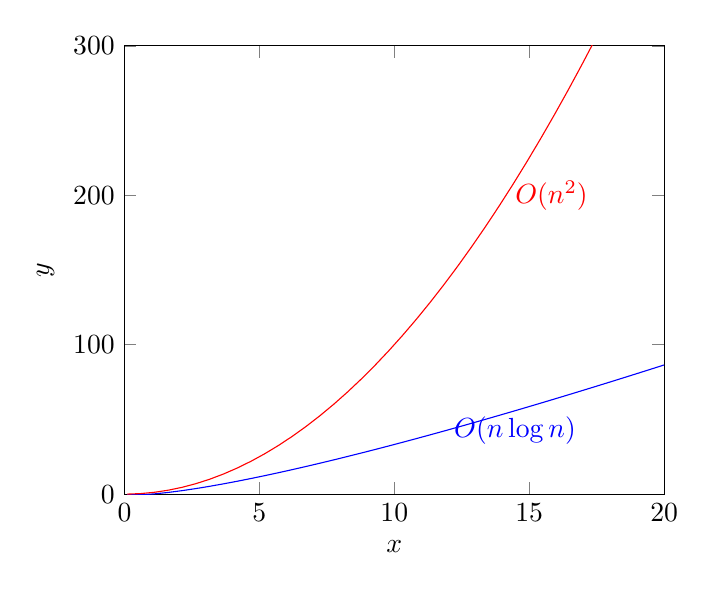
\begin{tikzpicture}
        \begin{axis}[ 
            xlabel=$x$,
            ylabel=$y$,
            xmin=0,
            ymin=0,
            ymax=300,
            xmax=20,
            samples=40,
            domain=0.1:20
            ] 
            \addplot[color=blue] {x * log2(x)} node[pos=0.5,anchor=west] {$O(n \log n)$};
            \addplot[color=red] {x^2} node[pos=0.5,anchor=west] {$O(n^2)$}; 
        \end{axis}
    \end{tikzpicture}
    \caption{grafico dell'equazione della complessita del algoritmo merge sort in confronto con il bubble sort}
\end{figure}
\section{Heap sort:}
L’Heap Sort è un algoritmo di ordinamento basato sulla struttura dati dell’heap binario. Il suo funzionamento si articola in due fasi principali: 
\begin{wrapfigure}{r}{0.3\textwidth}
        \begin{center}
            \animategraphics[loop,autoplay,scale=0.4]{10}{C:/Users/daniel/Desktop/algoritmi-ordinamento/relazione/media/Heapsort/Heap_sort2-}{0}{77}
        \end{center}
\end{wrapfigure}
la costruzione di un max-heap (o min-heap a seconda dell’ordinamento desiderato) e l’estrazione ripetuta del massimo (o minimo) elemento dall’heap per
ottenere la sequenza ordinata. Inizialmente, l’algoritmo trasforma l’array in un max-heap, garantendo che ogni nodo padre sia maggiore o uguale ai suoi 
figli. Successivamente, il massimo elemento, che si trova alla radice dell’heap, viene scambiato con l’ultimo elemento dell’array e l’heap viene riorganizzato
per ripristinare la proprietà dell’heap. Questo processo si ripete fino a ottenere un array ordinato
\subsection{Complessità:}
L’Heap Sort ha una complessità temporale di O(n log n) in tutti i casi, compresi il caso medio, peggiore e migliore. Durante la costruzione dell’heap, ogni 
elemento viene inserito con un costo massimo di log n operazioni, e l’estrazione di ogni elemento richiede anch’essa O(log n) operazioni. Questo lo rende 
una scelta efficiente per l’ordinamento di grandi dataset.

A differenza del Merge Sort, l’Heap Sort non richiede memoria aggiuntiva significativa, poiché opera in-place con O(1) di spazio extra. Tuttavia, non è 
un algoritmo stabile, il che significa che l’ordine relativo degli elementi uguali può essere alterato durante l’ordinamento. Inoltre, rispetto al Quick 
Sort, l’Heap Sort può avere prestazioni pratiche leggermente inferiori a causa di un accesso meno efficiente alla memoria, dovuto alla struttura ad albero dell’heap.
\begin{figure}[H]
    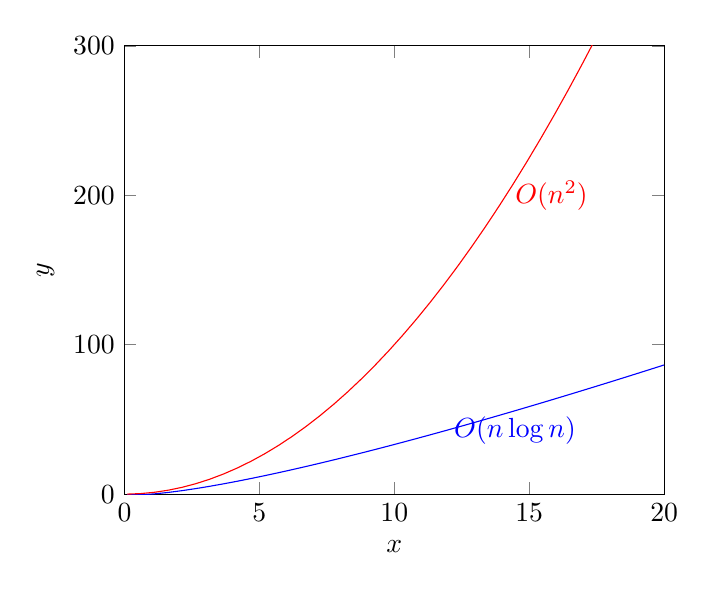
\begin{tikzpicture}
        \begin{axis}[ 
            xlabel=$x$,
            ylabel=$y$,
            xmin=0,
            ymin=0,
            ymax=300,
            xmax=20,
            samples=40,
            domain=0.1:20
            ] 
            \addplot[color=blue] {x * log2(x)} node[pos=0.5,anchor=west] {$O(n \log n)$};
            \addplot[color=red] {x^2} node[pos=0.5,anchor=west] {$O(n^2)$}; 
        \end{axis}
    \end{tikzpicture}
    \caption{grafico dell'equazione della complessita del algoritmo heap sort}
\end{figure}
\section{Insertion sort:}
\begin{wrapfigure}{r}{0.3\textwidth}
        \begin{center}
            \animategraphics[loop,autoplay,scale=0.44]{10}{C:/Users/daniel/Desktop/algoritmi-ordinamento/relazione/media/Insertionsort/insertionsort2-}{0}{238}
        \end{center}
\end{wrapfigure}
L’Insertion Sort è un algoritmo di ordinamento che costruisce la sequenza ordinata inserendo progressivamente ogni elemento nella posizione corretta rispetto 
agli elementi già ordinati. Funziona iterando sugli elementi della lista e spostando all’indietro quelli già ordinati per fare spazio all’elemento corrente 
nella sua posizione ideale. In questo modo, la lista viene ordinata gradualmente, come se si stessero ordinando delle carte in mano.
\subsection{Complessità:}
La complessità temporale dell’Insertion Sort è \(O(n²)\) nel caso medio e nel caso peggiore, poiché ogni elemento deve essere confrontato e potenzialmente
spostato rispetto agli elementi precedenti. Tuttavia, nel caso migliore, quando la lista è già ordinata, la complessità si riduce a \(O(n)\), rendendolo
molto efficiente per dataset piccoli o quasi ordinati. Un vantaggio dell’Insertion Sort è che è un algoritmo stabile e opera in-place con un consumo 
di memoria O(1), rendendolo adatto a situazioni in cui la memoria è limitata o si ha bisogno di un algoritmo semplice ed efficace per piccoli insiemi 
di dati. Inoltre, rispetto ad altri algoritmi di ordinamento più avanzati, l'Insertion Sort ha un overhead computazionale molto basso, rendendolo una 
scelta ottimale in scenari in cui il numero di elementi è limitato e le operazioni devono essere eseguite rapidamente.
\begin{figure}[h]
    \begin{tikzpicture}
        \begin{axis}[ 
            xlabel=$x$,
            ylabel=$y$,
            xmin=0,
            ymin=0,
            ] 
            \addplot {x^2}; 
        \end{axis}
    \end{tikzpicture}
    \caption{grafico dell'equazione della complessita del algoritmo Inserion}
\end{figure}
\section{Dati sperimentali:}
Dopo una serie di prove i tempi che gli algoritmi hanno impiegato sono i seguenti:
\begin{table}[h]
    \centering
    \caption{Tempi di esecuzione degli algoritmi di ordinamento}
    \begin{tabular}{lcccc}
    \toprule
    \textbf{Algoritmo} & \textbf{tempo impiegato} \\
    \midrule
    Bubble Sort & $O(n)$ \\
    Selection Sort & $O(n^2)$ \\
    Insertion Sort & $O(n)$ \\
    Merge Sort & $O(n \log n)$ \\
    Quick Sort & $O(n \log n)$ \\
    \bottomrule
    \end{tabular}
    \label{tab:sorting-algorithms}
\end{table}
\end{document}